\section{Diffusion equation and atomic models}

We have already discussed how diffusion can be model on a macroscopical base using non equilibrium thermodynamics obtaining interesting result both for the forms of the fluxes and of the diffusion constant. Now, we want to look at a more microscopic level trying first to describe how we can understand the motions of atoms looking at their density $c(\vb{x}, t)$ inside the material.

We have seen in the previous section how the flux of particles $\vb{J}$ can be described by using the density of atoms inside the material via Fick's first law, \eqref{eq:FickLaw}. Still, we can also try to describe the density of atoms inside the system, in fact the function $c$ describing the number of atoms inside the material will need to respect some continuity condition such as \eqref{eq:ContEquEntropy}. These two conditions taken together allow us to obtain a really powerful tool in order to study the evolution of density inside materials.
\thm{Second Fick's law}
{
    Inside a multicomponent material the density $c_i(\vb{x}, t)$ of the $i$-th component respect the following differential equation
    \begin{equation}
        \label{eq:SecFickLaw}
        \pdv{c_i}{t} = D_i \laplacian c_i.
    \end{equation}
}
\pf{Proof}
{
    We can write down the continuity equation for the densities assuming that source or sink terms $\dot{n}_i$ are negligible, since the vast majority of the time this is the case, so that we have
    \begin{equation}
        \pdv{c_i}{t} = -\grad\vdot\vb{J}_i = \grad\vdot\left( D_i\grad c_i \right).
    \end{equation}
    In general $D_i$ should be a tensor, still we are going to think at it as a simple scalar which in general can be assumed to depend on position through the density, as $D_i(c_i)$. Meaning that the diffusivity can be expanded using Taylor as
    \begin{equation}
        D_i \approx D(\left\langle c_i \right\rangle) + \left( c_i - \left\langle c_i \right\rangle \right)\eval{\pdv{D_i}{c_i}}_{\left\langle c_i \right\rangle},
    \end{equation}
    where $\left\langle c_i \right\rangle$ is the average value of the density inside the material and was chosen as the expansion point for simplicity. Inserting that expansion inside the continuity equation we get
    \begin{equation}
        \grad\vdot\left( D_i\grad c_i \right) = D(\left\langle c_i \right\rangle)\laplacian c_i + \eval{\pdv{D_i}{c_i}}_{\left\langle c_i \right\rangle} \left( \laplacian c_i + \grad c_i \vdot \grad c_i \right),
    \end{equation}
    but the second term is often neglected since the diffusivity has a general low dependence on the density, obtaining the wanted result.
}

\noindent
This equation allow us to describe the density of atoms inside the material in every moment in time given some initial conditions. To make an example, in 1D it's easy to see how if you take as a boundary condition for the density $c_i (x, t\to 0) = n_i\delta(x)$ than the following function is the solution
\begin{equation}
    c_i(x, t) = \frac{n_i}{\sqrt{4\pi D_it}}e^{-\frac{x^2}{4D_it}}.
\end{equation}
Where $n_i$ is the total number of atoms so that $c_i$ will be the number of atoms divided by a lenght, and one can easily see how that expression satisfy both the partial differential equation and the boundary conditions. From it, we can see how the atoms will start centered in the  origin and then will start to spread from it inside the material. In particular one can see how the average displacement of the atoms will be equal to the spread of the Gaussian itself $\sigma$ which can be easily computed using the known formula
\begin{align}
    \label{eq:Displ1D}
    &G(\mu, \sigma) = \frac{C}{\sqrt{2\pi\sigma}}e^{-\frac{(x - \mu)^2}{2\sigma^2}}, &\sigma = \sqrt{2D_it}.
\end{align}
Meaning that the average displacement will be proportional to $\sqrt{t}$, which is typical for diffusion phenomena showing how the process is slow needing much more time to spread the atoms as the dimensions of the system increase.

This result is general also when we look at higher dimensions, since it's possible to see that the same boundary condition and solution can be used even in 2D or 3D so that the solution is a simple product of the 1D one
\begin{equation}
    c_i(\vb{r}, t) = \frac{n_i}{\left( 4\pi D_it \right)^{d/2}}e^{-\frac{\vb{r}^2}{4D_it}}.
\end{equation}
Where $d$ is the dimensionality of the system, and we can see how the Dirac delta form for $t \to 0$ is still respected along with the differential equation. Also, the form of the average displacement is closer to the naive 1D case, but we can find out a more general form by evaluating it explicitly as
\begin{equation}
    \label{eq:DiffEquaModel}
    \left\langle R^2(t) \right\rangle = \frac{\int_{\mathbb{R}^+}\int_{\Omega}r^2c(r, t) r^2\dd \Omega\dd r}{\int_{\mathbb{R}^+}\int_{\Omega}c(r, t) r^2\dd \Omega\dd r} = 2dD_it,
\end{equation}
which is consistent with \eqref{eq:Displ1D}. This result is telling us that doesn't matter the dimension, the evolution of the displacement in a diffusive process only depend on the nature of the process itself and scales in time as $\sqrt{t}$, usually slow.

Therefore, using these results we were able to already describe some interesting properties of the diffusion process in a material having some important quantitative results. Still, this is only the beginning this model can be highly refined by using several considerations that will allow for it to be of great precision.

\nt
{
    The Gaussian form of the solution is interesting not only for the description of the evolution in time itself, but also on an experimental point of view. In fact, if one is able to evaluate $c(x, t)$ as function of position and time can see how
    \begin{equation}
        \ln c_i = const. - \frac{x^2}{4D_it},
    \end{equation}
    meaning that by making a linear fit in a $ln c_i$ vs $x^2$ plot at a certain time will allow us to estimate $D_i$ experimentally.
}

\subsection{Diffusion and random walk}

Another way to approach the modelling of diffusion is describing it using the mathematical model of the \textbf{random walk}. We can consider the atom moving by performing a series of possible jumps in space defined by the vectors $\{\vb{r}_i\}$, where every jump can be done with a frequency $\Gamma$. This means that after a certain time $t$ the number of jumps performed would be $\mean{N_{t}} = \Gamma t$ and the distance travelled by the atom would be
\begin{align}
    &\vb{R}(t) = \sum_{i=1}^{\Gamma t} \vb{r}_i, &R^2(t) = \sum_{i=1}^{\Gamma t} r_i^2 + 2\sum_{i=1}^{\Gamma t - 1} \sum_{j=1}^{\Gamma t - i} \vb{r}_i \vdot \vb{r}_{i+j}.
\end{align}
Where also the square of the displacement was reported since our aim is to evaluate the mean square displacement of the average walker inside the diffusion process and confront it with the previous model. Therefore, by taking the average of $R^2$ it's possible to see how it's value will take the form of
\begin{equation}
    \label{eq:RandWalkMod}
    \mean{R^2(t)} = \Gamma t\mean{r^2} + 2\mean{\sum_{i=1}^{\Gamma t - 1} \sum_{j=1}^{\Gamma t - i} \vb{r}_i \vdot \vb{r}_{i+j}} = \Gamma t\mean{r^2} + 2\Pi(t),
\end{equation}
where $\Pi$ is the time correlation function between the jumps, describing how much the jumps influence one another. Now, in the case of a pure random walk, the jumps are totally uncorrelated with a uniform probability of going in every possible direction. Meaning that $\Pi = 0$ and average displacement takes a form analogous to the one already seen
\begin{align}
    &\mean{R^2(t)} = \Gamma t\mean{r^2},
\end{align}
showing how the evolution is still proportional to $t^{1/2}$ as expected from diffusion.

We can now confront the model just obtained, \eqref{eq:RandWalkMod}, and the more macroscopic description given by the solution of the diffusion equation, in \eqref{eq:DiffEquaModel}, and see how we can retain a form for the diffusivity.
\thm{Microscopic diffusivity}
{
    Inside an atomistic model the diffusion can be though as a random walk with frequency of jump $\Gamma$, so that macroscopically the density can be described using FIck's law with a diffusivity given by the microscopic properties as follows 
    \begin{align}
        \label{eq:MicroDiff}
        &D = \frac{\Gamma\mean{r^2}f}{2d}, &f = 1 + \frac{2\Pi(t)}{\Gamma t\mean{r^2}},
    \end{align}
    where $\Pi(t)$ is the time correlation function for the jumps.
}
\pf{Proof}
{
    At first, we can see how \eqref{eq:RandWalkMod} can be recast in a simpler form analogous to the one in \eqref{eq:DiffEquaModel} by using
    \begin{align}
        &\mean{R^2(t)} = \Gamma t\mean{r^2}f, &f = 1 + \frac{2\Pi(t)}{\Gamma t\mean{r^2}}.
    \end{align}
    Which can be confronted with the mean square displacement of the macroscopic diffusion model to see that
    \begin{equation}
        D = \frac{\Gamma\mean{r^2}f}{2d},
    \end{equation}
    having our final result.
}
\noindent
Therefore, by simple consideration on the microscopic nature of the diffusion mechanism we were able to connect the diffusivity to the rate of jump inside the lattice. All we have to do now is describe how such rate can be expressed quantitatively, and then the whole model would be complete.

\subsection{Thermally activated jumps}

We now consider a statistical model to evaluate the transition rate of the jump between the different main states inside the material, starting from a minimum and jumping to a maximum, called transition state, to then go into another minimum, as depicted in \figref{fig:ThermAct}. In particular, we are going to make some important assumption in order to work out the model:
\begin{enumerate}
    \item[1)] Single particles in a potential energy with harmonic wells, 
    \item[2)] Thermal equilibrium described by classical partition function, 
    \item[3)] Quantum tunneling is negligible.
\end{enumerate}
Using this assumption is possible to create a microscopic model that allow us to obtain a quantitative evaluation of the transition rate that is given by the following result.
\thm{Thermally activate transition rate}
{
    A thermal activated process inside a system where quantum tunneling is negligible posses a transition rate that can be expressed with the form
    \begin{align}
        &\Gamma = z\nu\exp\left( -\frac{E^m}{k_BT} \right), &\nu = \frac{1}{2\pi}\sqrt{\frac{\beta}{m}}.
    \end{align}
    Where $E^m$ is called \textbf{migration energy}, defined as the difference between the energy of the minimum of the starting point and the transition point energy, while $\beta$ is the first order coefficient of the Taylor expansion on the minimum and $z$ the numbers of neighboring sites.
}
\begin{figure}[t]
    \centering
    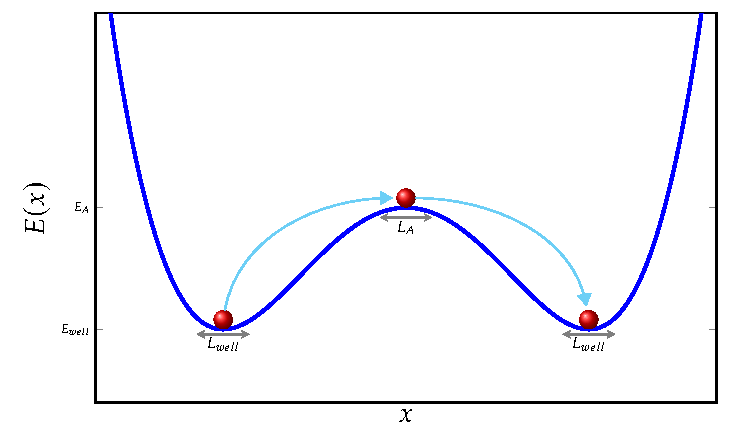
\includegraphics[width=0.8\textwidth]{Immagini/ThermAct.pdf}
    \caption
    {
        Representation of the energy landscape of a possible system under study in the context of thermally activated processes. Where the path followed by the atom is in 1D and is described by the directions of the arrows.
    }
    \label{fig:ThermAct}
\end{figure}
\pf{Proof}
{
    From the assumption we can evaluate the value of the medium time for a transition to happen as the quantity
    \begin{align}
        &\tau_{cross} = \frac{L_A}{\mean{v}}, &\mean{v} = \frac{\int_{\mathbb{R}^+} ve^{-\frac{mv^2}{2k_BT}} \dd v}{\int_{\mathbb{R}^+} e^{-\frac{mv^2}{2k_BT}} \dd v} = \sqrt{\frac{2\pi m}{k_BT}},
    \end{align}
    where a Maxwell-Boltzmann distribution for the velocities was used in the computations of the mean. So, the value of $1/\tau_{cross}$ will give us the probability of a particle to cross the energy barrier in the unit time, now to complete the probability of transition we need the probability of having a particle to be ready to jump, which can be given by
    \begin{equation}
        P_{A} = \frac{N_A}{N_T} = \frac{N_A}{N_A + N_{well}} \approx \frac{N_A}{N_{well}} = \frac{Z_A}{Z_{well}}.
    \end{equation}
    Where $Z_A$ and $Z_{well}$ are the partition functions of the well and transition state of the one-particle system, also we assumed that the number of particle in the minimum are much larger that the one in the transition state. Now, the value of the partition function can be evaluated by assuming that the minimum has an energy that can be approximated using $E(x_{well}) = E_{min} + \beta(x - x_{well})^2$ while the maximum is nearly constant in the $L_A$ distance having that
    \begin{equation}
        \frac{Z_A}{Z_{well}} = \frac{\int_{-L_A/2}^{L_A/2} e^{-\frac{E(x)}{k_BT}}\dd x}{e^{-\frac{E_{min}}{k_BT}}\int_{-L_{well}/2}^{L_{well}/2} e^{-\beta\frac{(x - x_{well})^2}{k_BT}}\dd x} \approx L_Ae^{-\frac{E_A - E_{min}}{k_BT}}\sqrt{\frac{\beta}{2\pi k_BT}}.
    \end{equation}
    Where we also assumed that the integral over the well could be extended to the all domain in order to count also for the tails and have an analytic form for the solution. Therefore, we can so define $\Gamma'$ as the following quantity 
    \begin{equation}
        \Gamma' = \frac{P_A}{\tau_{cross}} = \frac{Z_A}{Z_{well}}\frac{1}{\tau_{cross}} = \nu e^{-\frac{E^m}{k_BT}},
    \end{equation}
    which represent the transition rate in a specific direction in space, since the model was in 1D, in reality the hopping can happen in all the possible directions of neighboring sites. Assuming that the probability of going in equivalent sites near the well has same $\Gamma'$ rates we need to sum all them up in order to obtain the total one, finding out the final result as claimed.
}
\noindent
We can see how the transition rate obtained in this particular one particle model is interesting, having a frequency multiplied by an exponential factor that goes down as the potential barrier needed to overcome the jump increases. Such a form allows us to give a simple and strong physical interpretation to the result, where the particle in equilibrium \textbf{vibrates on the minimum} with a changing intensity over time such that has a \textbf{non-zero possibility of vibrate with enough strength in order to overcome the barrier and hope}. Meaning that, in average, all particles stay in an equilibrium position for a time $1/\Gamma$ before hopping to another minimum inside the lattice due to thermal vibrations. Also, it's possible to see how the latter posses a typical amplitude $\nu\propto m^{-1/2}$ as expected from classical vibrations, meaning that also the \textbf{mass of the atom} gives a contribution, so that different isotope of the same element have different diffusive behaviors. This phenomenon created what takes the name of \textbf{isotope effect}.

Such a model is so able to describe the on a first principle base the very nature of the hopping as a statistical process, giving a quantitative evaluation of the transition rate that is at the very core of really important mechanism such as chemical reactions, not only atoms' diffusion. For this reason such theory, called \textbf{transition state theory}, is of great interest not only on a theoretical point of view and has been refined over time to also include the presence of many particles inside the system, relaxing the single particle assumption. We have not the time to undergo the study of such a complex theory, nevertheless we are going to make use of its result so that we are going to use the following form for the transition rate.
\cor{Many-body case}
{
    If we relax the condition of a single particle inside the system imagining to have a many-body interacting one, the transition rate take the following form
    \begin{equation}
        \label{eq:MBtransRate}
        \Gamma = z\nu\exp\left( -\frac{G^m}{k_BT} \right) = z\nu\exp\left( \frac{S^m}{k_B} \right)\exp\left( -\frac{H^m}{k_BT} \right).
    \end{equation}
} 
\noindent
Basically the energy of migration is exchanged with the free energy of migration. We can so use such a model for the transition rate to give out a final form that we can use for the diffusivity constant, since by inserting \eqref{eq:MBtransRate} into \eqref{eq:MicroDiff} we can obtain
\begin{equation}
    D = \frac{z\mean{r^2}f}{2d}\nu\exp\left( \frac{S^m}{k_B} \right)\exp\left( -\frac{H^m}{k_BT} \right).
\end{equation}
Which is the final microscopic form for the diffusivity where we can see how such a complex parameter depend on sever factors. The \textbf{geometry} of the system defined by the neighboring sites, $z$, the dimensionality and the correlation, $d$ and $f$. Then, \textbf{vibrations} with their general value of $\nu$ and \textbf{migration entropy} give a contribution, which in general is not too high having that often such factor are kept constant to reference values with right order of magnitude. At last, the most important contribution is given by the \textbf{migration enthalpy} which is generally the factor that influences the most the value of $D$, having not only a strong dependence on temperature, showing how the process is \textbf{thermally activated}, but also since its value can be high.

\ex{Vacancy diffusion}
{
    A simple example of application of such an equation is the case of diffusion of vacancy inside a fcc lattice. We know how $z = 12$ inside such a geometry and the distance between neighbors is $a/\sqrt{2}$, where $a$ is the lattice constant, meaning that $\mean{r^2} = a^2/2$. If we assume that the jumps are uncorrelated for the movement of a vacancy inside a lattice then we can easily see how the final form for the diffusivity is
    \begin{equation}
        D_V = a^2 \nu \exp\left( \frac{S^m_V}{k_B} \right)\exp\left( -\frac{H^m_V}{k_BT} \right).
    \end{equation}
    Such an equation gives us a lot of information, especially since we can experimentally evaluate $D$ at different temperatures so that by fitting $\ln D$ vs $1/T$ we can estimate $H^m_V$ which can be compared to first principle DFT computations of such value.

    Inside such systems we can also rephrase the motion of vacancies in terms of motions of atoms inside the material, since as a vacancy move also an atom follows along. Therefore, we can simply think at the jumping rate of atoms as the one of vacancy multiplied by the probability of having vacancies to move in, so that
    \begin{equation}
        \Gamma_A = \Gamma_V \frac{N_V}{N_T} = \Gamma_V X_V.
    \end{equation}
    We know analytic expressions for both of the quantities, so that we can write down the general form of the diffusivity but still we need first to say that in reality the diffusion of atom is not totally uncorrelated. In particular, we have that an atom jumping into a vacancy leaves behind another one, so that the probability of jump back into the other vacancy is higher than to wait for another one to show up, creating a correlation factor of $f \approx 1 - 2/z$. Using that and \eqref{eq:VacancyPresence} we can so obtain the following form
    \begin{equation}
        D_A = fa^2\nu\exp\left( \frac{S_V^m + S_V^f}{k_B} \right)\exp\left( -\frac{H_V^m + H_V^f}{k_BT} \right) = D_A^0e^{-\frac{E}{k_BT}},
    \end{equation}
    where $S_V^f$ and $H_V^f$ are the entropy and enthalpy of formation for the vacancy inside the material. It's also good to see how in general $D_A^0 \approx \SI{0.1}{}-\SI{1.0}{cm^2\second^{-1}}$, in good agreement with the typical values of $a \approx \SI{3}{\angstrom}$, $\nu \approx \SI{1e13}{\second^{-1}}$ and $S_V^m + S_V^f \approx 2k_B/\text{atom}$. 
}
\nt
{
    Such a model can effectively be tested in experiment using different types of setups, some examples are on slides, allowing for the evaluations both $H_V^m$ and $H_V^f$, which are incredibly important for testing theoretical first principle computations. In particular, it's also interesting to see how such values are highly correlated to other ones, like formation enthalpy is correlated to \textbf{cohesive energy}, since stronger are the bonds in the material the more difficult create a vacancy is. Another interesting one is the fact that migration enthalpy is related to the \textbf{bulk modulus}, which tells us how difficult is to move an atom in the material, and it makes sense since $H_V^f$ tells us the variation of the energy in the material when a vacancy travels inside it moving atoms on the way.
}

\subsection{Diffusion in ionic materials}

One of the most interesting application of diffusion in modern times is the understanding of how ions move inside materials, since ions are able to transport charge allowing for the creation of batteries. In fact, modern Lithium batteries uses Li ions as charge transports from anode to cathode making them diffuse inside liquid electrolyte, which allow for quick diffusion but at the risk of highly flammable batteries that can work only in a short range of temperatures. This lead to a lot of effort to substitute the organic electrolyte into a solid one making Li diffuse inside a material. We shall see how this is possible and how would also allow for high performance batteries to be created.

In order to understand it we shall need first to address the study of a general reaction inside the material. For example take the following situation
\begin{equation}
    n_1^r R_1 + n_2^rR_2 + \dots + n_N^rR_N \rightleftharpoons n_1^p P_1 + n_2^pP_2 + \dots + n_M^pP_M,
\end{equation}
where $n^r_i$ and $n^p_i$ are the mole of all the reactant needed and product created. We can have a look at the thermodynamic of such a reaction and describe its chemistry finding out a really important result.
\thm{Van't Hoff equation}
{
    In every reaction is possible to define an equilibrium constant $K_{eq}$ that describes the if the reaction is more favored in the direction of reactants or products, defined as
    \begin{equation}
        K_{eq} = \frac{\prod_{i=1}^M \gamma_i^p X_i^p}{\prod_{j=1}^N \gamma_j^r X_j^r} = \frac{\prod_{i=1}^M a_i^p}{\prod_{j=1}^N a_j^r},
    \end{equation}
    where the molar fractions are the one when the system is in thermal equilibrium. Such a constant is related to the free energy of the unmixed system, and at equilibrium we have that 
    \begin{align}
        &\Delta G^0 = -RT\ln K_{eq}, &K_{eq} = \exp\left( -\frac{\Delta G^0}{RT} \right).
    \end{align}
}
\pf{Proof}
{
    We can start by writing down the form of the $\Delta G^0$ in a simple known way by using the form
    \begin{equation}
        \Delta G^0 = \sum_{i=1}^M n_i^p\mu_{i}^{p0} - \sum_{i=1}^N n_j^r\mu_{j}^{r0}.
    \end{equation}
    Then, we know that in the case where the various reactants and product start mixing forming a solution we can use another known form for the Gibbs free energy that looks like this
    \begin{equation}
        \Delta G = \sum_{i=1}^M n_i^p\left( \mu_{i}^{p0} + RT\ln a_i^p \right) - \sum_{i=1}^N n_j^r\left( \mu_{j}^{r0} + RT\ln a_j^r \right) = \Delta G^0 + RT \ln K.
    \end{equation}
    Where $K$ is not equal to $K_{eq}$ since the molar fractions can be different from the two, and the equilibrium in the reaction is reached only when the number of products and reactants are so that $K = K_{eq}$. To found out such a value we can simply impose the equilibrium inside the solution by assuming that $\Delta G = 0$ and finding out the wanted results.
}
\noindent
This is a powerful result that allow us to see a lot of information on the reaction itself only by looking at the equilibrium constant. In particular, it's possible to see how if $K < K_{eq}$ then $\Delta G > 0$ and the products will decompose to generate reactants, instead for $K > K_{eq}$ the reactants will generate products.

The Van't Hoff equation will be able to give us key information for describing the concentration of defects inside ionic crystals. In fact, the real difference from the diffusion in a normal or ionic material is the presence of atoms that carries a charge since anions and cations are present in equal amount inside the latter. Therefore, we can't really have the simple formation of vacancies inside ionic material since would mean that by eliminating a charge the total material would no more be neutral and that cannot be. Such a constraint make so that the type of defects present inside such materials needs to be more complex to maintain the total charge having that typically are of two types: \textbf{Schottky}, where an anion and a cation leaves the structure together leaving two vacancies but no accumulated charge, \textbf{Frenkel}, a cation takes an interstitial position leaving a vacancy in its place. Thus, our next tusk will be, understand how much of such complex defects are present in the material and to do it we will use also a powerful notation that will help us in the reasoning.
\dfn{Kroger-Vink notation}
{
    We can write down a point defect inside an ionic crystal by using the form \ce{X_S^C}, where the various letters have the following meanings:
    \begin{itemize}[align=left, leftmargin=*]
        \item[\textbf{X}] is the element inside the defect, if a vacancy is present the letter V can be used or the symbol $\Box$;
        \item[\textbf{S}] is the site that the defects has taken place in, can be used the name of the atom that has substituted for example;
        \item[\textbf{C}] is the effective charge that the defect has inserted inside the system. For example, if a \ce{Cl^{+1}} is substituted by a vacancy its like having a negative charge more inside the material so that the defect is written as $\text{V'}_{\text{Cl}}$ where the apostrophe indicates $-1$. To write $+1$ a dot is used instead.  
    \end{itemize}
}